\section{Causal Inference Algorithms}
\label{sec:5}
Causal inference consists of two key ideas to estimate causal relations between events: removing spurious correlations and determining directions of causal edges. This section explains the basic idea of causal inference and existing approaches to analyzing log data. I will illustrate three main classes of algorithms: constraint-based, score-based, and functional-based. In this paper, I selected one prominent algorithm from each group. But if we start exploring the multivariate time-series analysis literature regarding causality, we will likely come across Granger causality. This paper will also explain Granger causality and why it is not the true causality, unlike "cause and effect" relationships.
\subsection{Constraint-based}
The primary and main idea of a theory of inferred causation is to present a causal structure among variables in an acyclic-directed graph (DAG) called a causal graph in which arrows indicate causal orders, where each node represents a feature from the data set \cite{pearl2009causality}. If we want to say that $X$ causally influences $Y$ and not vice versa, we write $X \rightarrow Y$. \newline

But firstly, I will define the statistical decision procedure, a hypothesis test for \textbf{conditional independence}, to reveal causality from correlation. Conditional independence is usually formulated in terms of conditional probability. Assume three events: $X$, $Y$, and $Z$. $X$ and $Y$ are conditionally independent for given $Z$ if
\begin{equation}
P(X \mid Y, Z)=P(X \mid Z)
\end{equation}
where the events $X$ and $Y$ are independent as long as $Z$ appears. In other words, since the probability of $X$ given $Z$ is the same as the probability of $X$ given both $Y$ and $Z$, this equality expresses that $Y$ contributes nothing to the certainty of $X$. With conditional independence, we can remove pseudo-causality/spurious correlation in this way. \newline
\begin{figure}[ht]
\centering
    \label{fig:ci-example}
    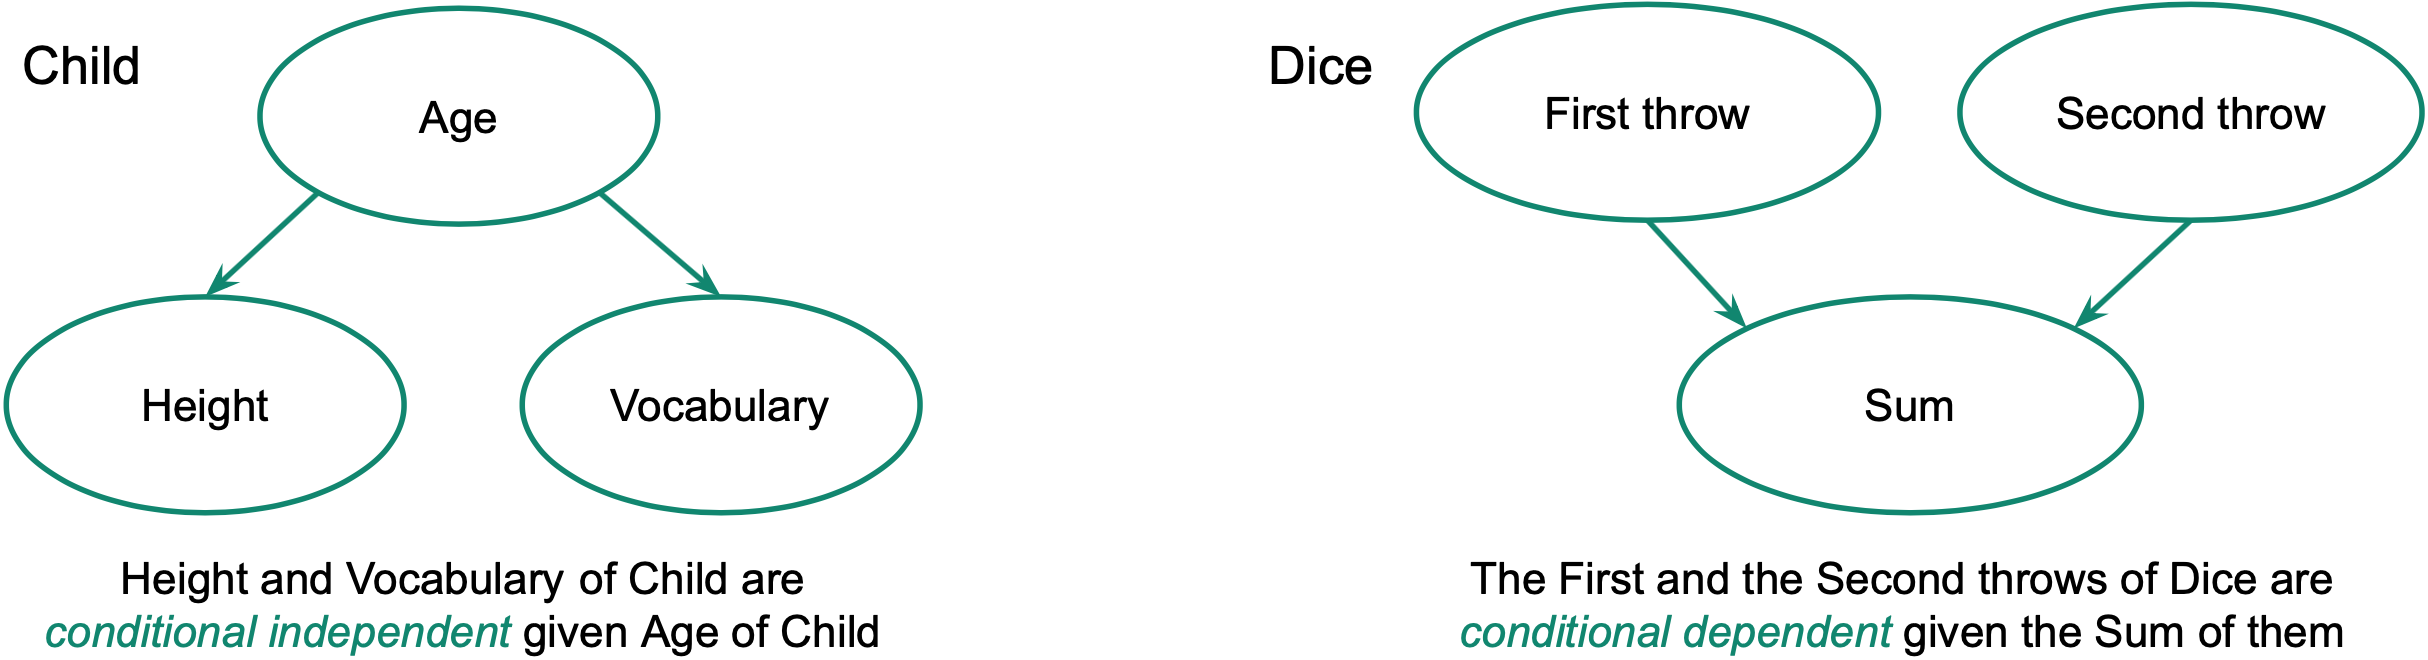
\includegraphics[width=\textwidth]{figures/ci_example.png}
    \caption{The conditional independence examples.}
\end{figure}

To clarify, neither conditional independence of two variables implies their independence nor vice versa. I prepared two counterexamples (see also Figure \hyperref[fig:ci-example]{5}). The first example is about a child. Firstly, we focus only on the child's height and the number of words the child knows. When the first parameter is high, the second is high, too. So, they are not independent. But if we provide the child's age. We will see the dependence between age and height and between age and vocabulary. But if we go back to the probability definition, we can say that the height and vocabulary of the child are conditionally independent, given the child's age. The second example is about dice. We can throw dice twice and get two separate results. But if we provide the parameter like the sum of these throws, we will see the pairwise dependency between each throw and sum. And we can say in this case that the first and the second throw of dice are conditionally dependent on their sum. \newline

One can consider three methods for testing conditional independence in practice \cite{kobayashi2017mining}:
\begin{enumerate}
\item The \textit{G-square test} is a method to evaluate conditional independence of binary or multi-level data based on information theory, using conditional cross-entropy ($CE$) and the data length ($m$). The G-square statistic $G^2$ is defined as:
\begin{equation}
G^{2}=2 m C E(X, Y \mid Z)
\end{equation}
\item The \textit{Fisher-Z test} evaluates the conditional independence of continuous data based on Pearson's correlation coefficient ($r$) and the data length ($m$). The statistic $Zs$ is defined as:
\begin{equation}
Z s=\frac{\sqrt{m-|Z|-3}}{2} \log \frac{1+r}{1-r}
\end{equation}
\item The \textit{conditional mutual information test} evaluates conditional independence of discrete and continuous data based on information theory, using conditional entropy and probability function. The conditional MI test $I$ is defined as:
\begin{equation}
I(X , Y \mid Z)=H(X \mid Z)-H(X \mid Y, Z)=E\left[\log \frac{p(X, Y \mid Z)}{p(X \mid Z) p(Y \mid Z)}\right]
\end{equation}
\end{enumerate}
In experiments with log data, Kobayashi et al. \cite{kobayashi2017mining} found that Fisher-Z leaves more false-positive edges and takes more time than the G-square test. \newline

This class of algorithms relies on four assumptions to develop the correct DAG structure. All the independencies in a graph need to be under the conditional independence criterion \cite{nogueira2021causal}:
\begin{enumerate}
\item \textit{Causal Markov} – if two variables are conditional independent of each other, they must be unconnected given all their intermediate variables.
\item \textit{Causal Faithfulness} – if two variables are conditionally dependent, connecting those variables must be an edge.
\item \textit{Causal Sufficiency} – all the common causes of a pair of variables are measured (no hidden/external causes).
\item \textit{Independency} –  no variable is an (indirect) cause of itself.
\end{enumerate}

Constraint-based methods for causal discovery have the advantage of being generally applicable. Still, the disadvantages are that faithfulness is a strong assumption and may require substantial sample sizes to get good conditional independence tests.
\begin{figure}[H]
\centering
    \label{fig:pc}
    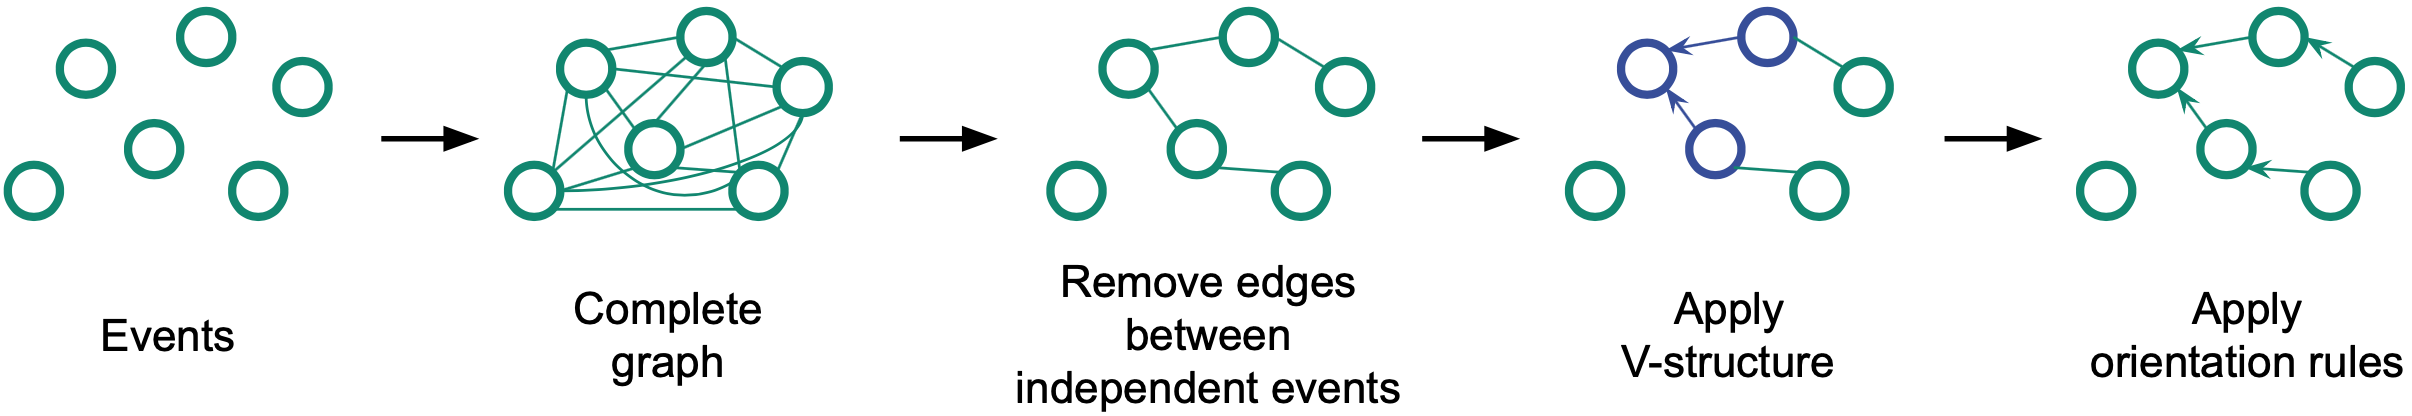
\includegraphics[width=\textwidth]{figures/pc.png}
    \caption{The PC algorithm flow.}
\end{figure}
\textbf{PC Algorithm} \cite{spirtes2000causation}. One of the most common algorithms in literature is the PC algorithm, which aims to find the graphs representing precisely the independent relationships in the data through hypothesis tests. The PC algorithm consists of four steps (see also Figure \hyperref[fig:pc]{6}). We start with a set of created from logs event time-series. Then, we construct a complete (fully connected undirected) graph from events. Next, we eliminate edges between conditionally independent nodes by analyzing all pairs. Then, the triple of nodes (in blue color on Figure \hyperref[fig:pc]{6}) is called V-structure with the following orientations of edges. So, we look for the V-structures of nodes and determine the edge direction. Finally, we determine other edge directions with the orientation rules defined by the algorithm. However, some edges can be undirected even after applying the PC algorithm if one does not have enough information to determine edge directions. In other words, in the first two steps, we estimate a skeleton graph that is an undirected causality graph with the idea of causal inference. In the last two steps, we determine the directions of the detected edges with established rules. The V-structure is the main rule to decide on the direction of an edge. For example, three events $X$, $Y$, and $Z$ are part of a graph $X-Y-Z$. $X$ and $Y$ are correlated, and $Y$ and $Z$ are connected. One obtains a causal relationship $X \rightarrow Y \leftarrow Z$ if $X$ and $Z$ are not conditionally independent for $Y$. The remaining undirected edges can be oriented using experimental data or knowledge about data sources. \newline

In practice, the PC algorithm has some variations. One of these algorithms is the PC-stable \cite{colombo2014order}. This algorithm solves the problem that the traditional PC depends on the order in which the events are given to the algorithm. This adaptation modifies how the algorithm creates the skeleton: in each level, the events that should be removed are saved in a queue and only permanently removed in the next iteration. PC-simple modification is based on local causality discovery \cite{buhlmann2010variable}. The difference is that it only analyses the strongly related variables to the selected target variable (that is, it does not analyze or create the network with the remaining variables). This algorithm was developed to deal with high-dimensional data. The HITON-PC combines two previously presented algorithms, PC-stable and PC-simple \cite{aliferis2003hiton}. Another extension is the parallel-PC, which is a parallel adaptation of PC \cite{le2016fast}. This parallelization is done in the conditional independence tests performed at each algorithm level. These tests are grouped and distributed in different cores. The MPC modifies the original orientation rules by adding a new rule that prevents the creation of cycles (although DAGs do not allow cycles, PC does not explicitly prevent their creation) \cite{tsagris2019bayesian}.
\subsection{Score-based}
These algorithms differ from the previous ones because they are based on the greedy strategy to make the locally optimal choice at each stage and compare the interim graphs through the Bayesian Information Criterion (BIC) \cite{stoica2004model}. These algorithms are usually costly in terms of performance since they have to score every model.
\begin{figure}[H]
\centering
    \label{fig:ges}
    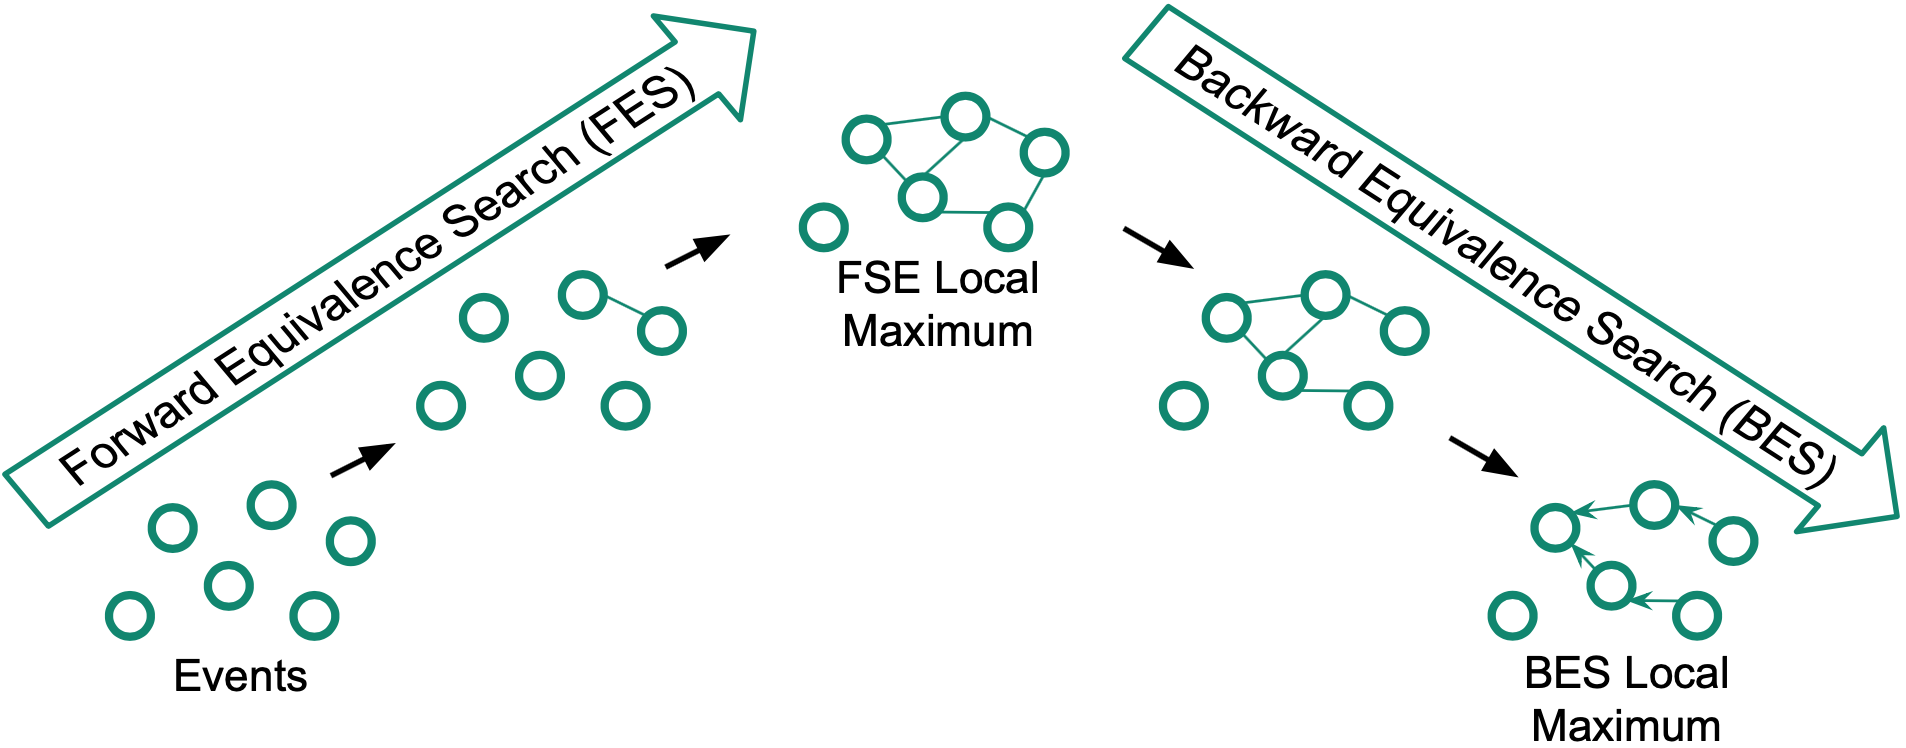
\includegraphics[width=\textwidth]{figures/ges.png}
    \caption{The Greedy Equivalence Search flow.}
\end{figure}
\textbf{Greedy Equivalence Search (GES)} \cite{chickering2002optimal}. The GES algorithm generally consists of two phases (see also Figure \hyperref[fig:ges]{7}). In the Forward Equivalence Search (FES) phase, the algorithm starts with a set of events. Then, at each step, as a decision is made whether adding an edge to the graph will increase the score BIC, the edge that most improves the score is added until the algorithm reaches a local maximum. This algorithm analyses all possible node-neighbors each time. Then, the second phase of the algorithm begins, which asks, edge by edge, which edge removal, if any, will improve the score until it reaches a local maximum. But in this phase, the direction of the edges is also considered. \newline
	
In practice, the GES algorithm also has some variations. One example is the Greedy Interventional Equivalence Search (GIES), in which, besides the FES and BES phases, there is a third phase called the Turning Step \cite{hauser2012characterization}. In this extra phase, the algorithm iterates all possible orientations of edges without losing edges or creating new ones so that the previous graph can be reconstructed by only changing arrows. This phase was added with the intent to enhance estimation. Another example is the Fast Greedy Equivalence Search (FGS) \cite{ramsey2017million}. This algorithm uses parallelization to optimize the original GES and applies a limited faithfulness assumption.
\subsection{Functional-based}
\begin{figure}[H]
\centering
    \label{fig:x-y}
    
\includegraphics[width=0.3\textwidth]{figures/x_y.png}
    \caption{The simple causal graph.}
\end{figure}
For the introduction to this class, I will start with defining the problem by determining the causal direction in the two-variable case, where no conditional independence relationship is available. A fundamental issue is given two variables $X$, $Y$ (see also Figure \hyperref[fig:x-y]{8}), how to distinguish cause from effect. To do so, we must find a way to capture the asymmetry between them. Functional-based approaches represent the effect $Y$ as a function of the direct causes $X$ and some unmeasurable factors or noise:
\begin{equation}
Y = f(X) + E
\end{equation}
where $E$ is assumed to be independent of $X$, the function $f$ explains how $Y$ is generated from $X$. We assume that the transformation from $(X, E)$ to $(X, Y)$ is invertible, so $E$ can be uniquely recovered from the observed variables $X$ and $Y$. So, these algorithms consider the data asymmetry effect induced by the causal directions \cite{glymour2019review}.
\begin{figure}[H]
\centering
    \label{fig:fb-example}
    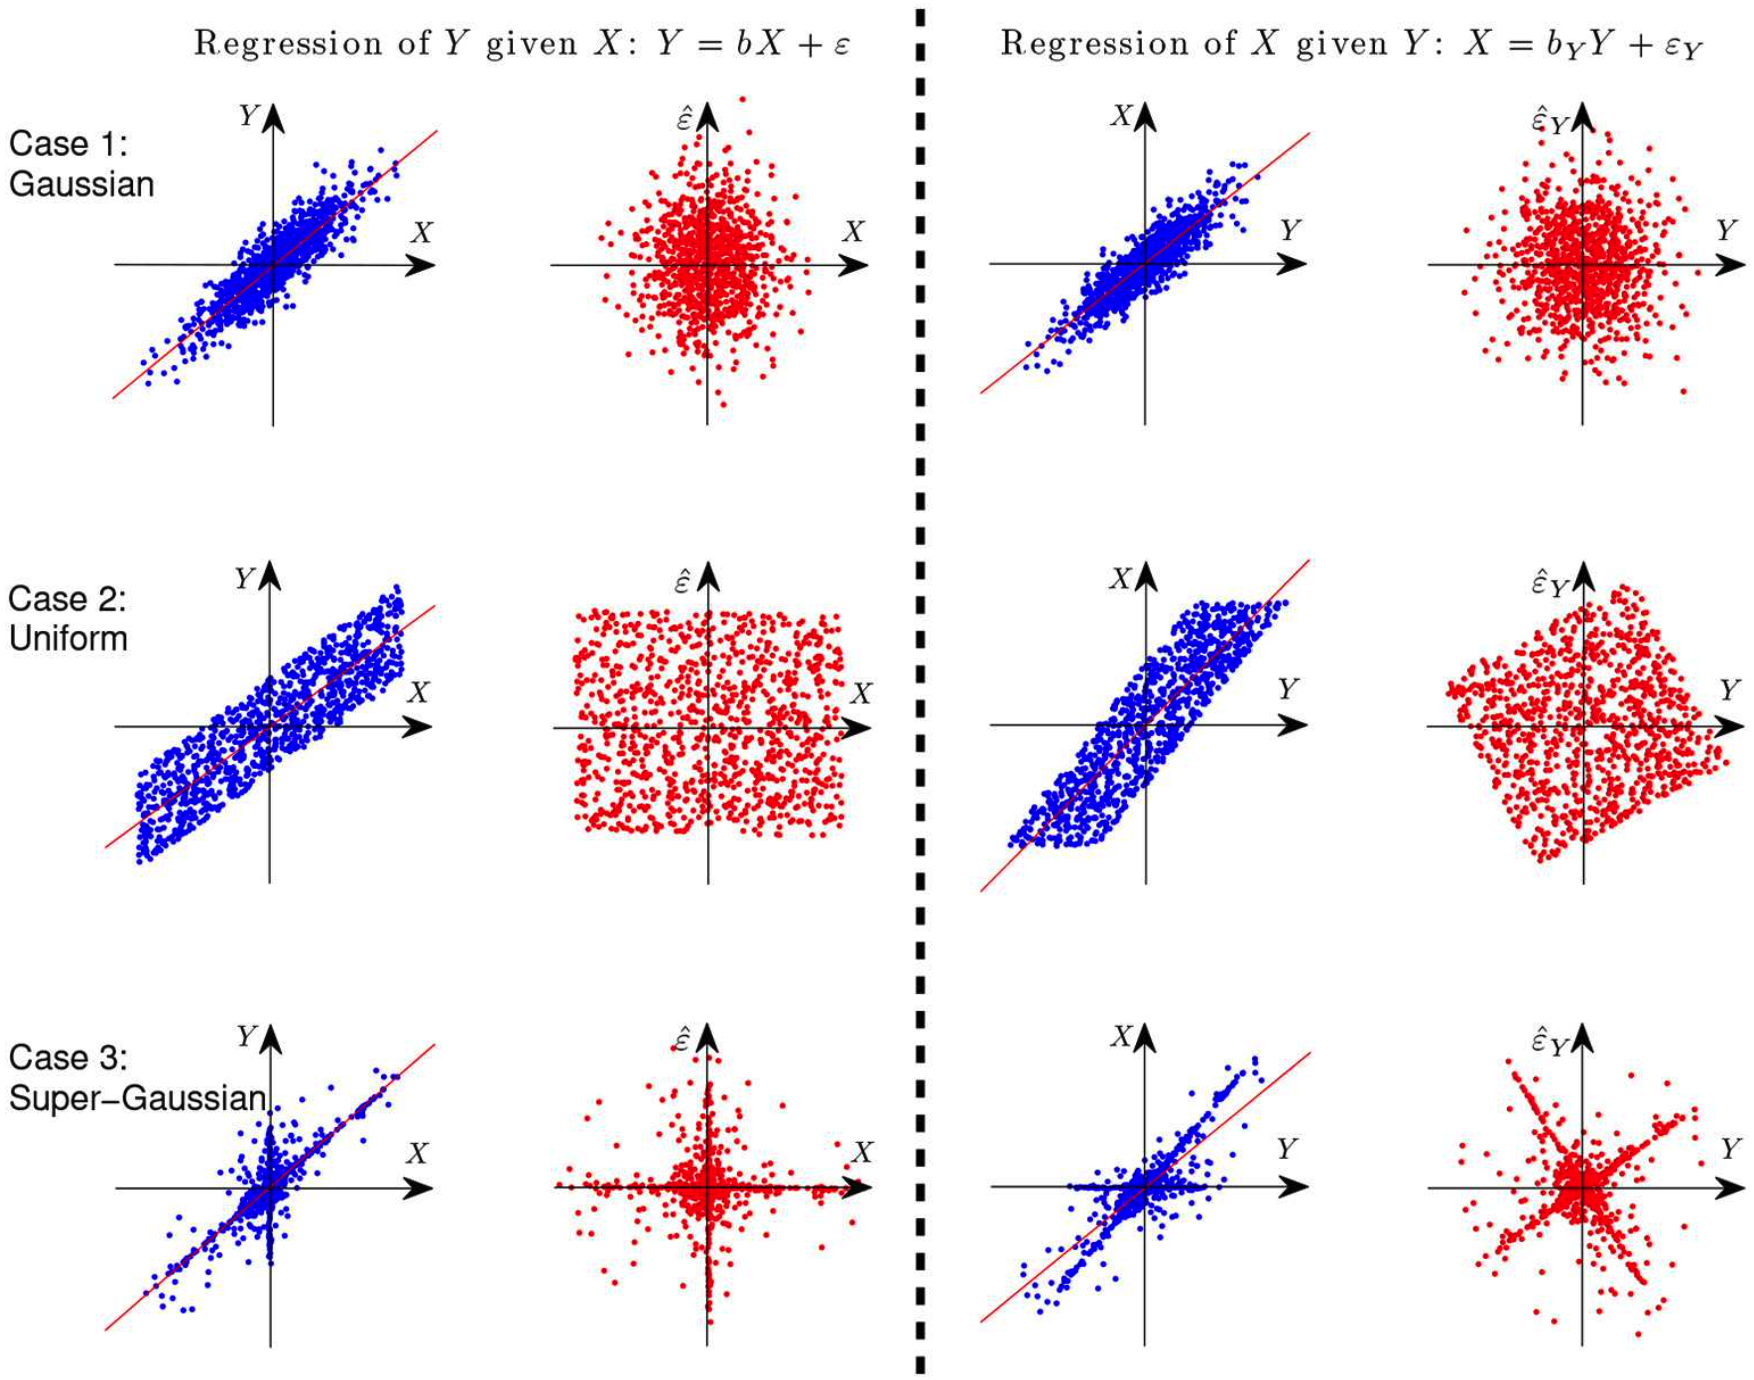
\includegraphics[width=\textwidth]{figures/fb_example.png}
    \caption{The illustration of causal asymmetry between two variables with linear relations.}
\end{figure}
What does it mean by the data asymmetry effect? Under the above assumptions, we fit the functional-based test and then check for independence between the estimated noise term and the hypothetical cause. So, the direction that gives an independent noise term is considered plausible. The figure \hyperref[fig:fb-example]{9} is a simple example of why it is possible to identify the causal direction between two variables in the linear case, $f$ is the linear function. Assume $Y$ is generated from $X$ in a linear form, where $E$ is independent of $X$. Columns 1 and 3 are the scatter plots of the two variables $X$, and $Y$, the red line is the linear regression of $Y$ on $X$, and columns 2 and 4 are the predictor and regression residual for two different regression tasks. The three rows correspond to different settings: $X$ and $E$ are both Gaussian (case 1), uniformly distributed (case 2), and distributed according to some super-Gaussian distribution (case 3). In the last two cases, $X$ and $E$ are non-Gaussian, and one can see clearly that for regression of $X$ given $Y$ (the backward direction), the regression residual is no longer independent of the predictor. However, they are uncorrelated by the construction of regression. In other words, in those two situations, the regression residual is independent of the predictor only for the correct causal direction, giving rise to the causal asymmetry between $X$ and $Y$. As a result, based on this asymmetry, we can conclude that $X$ is the cause of $Y$ \cite{glymour2019review,goudet2018learning}.\newline

In practice, there are two directions of functional-based methods. The first way uses a linear function (e.g., Linear Non-Gaussian Acyclic Model (LiNGAM) \cite{shimizu2006linear}), and the second way — non-linear functions (e.g., Post-nonlinear (PNL) Causal Model \cite{zhang2012identifiability}). In the linear, non-Gaussian, and acyclic model (LiNGAM), a function is linear, and at most, one of the noise terms $E$ and cause $X$ is Gaussian. In PNL, the effect $Y$ is further generated by a post-nonlinear transformation on the non-linear effect of the cause $X$ plus noise term $E$, where both functions are non-linear, and the outer function is assumed to be invertible.
\begin{figure}[H]
\centering
    \label{fig:fb-flow}
    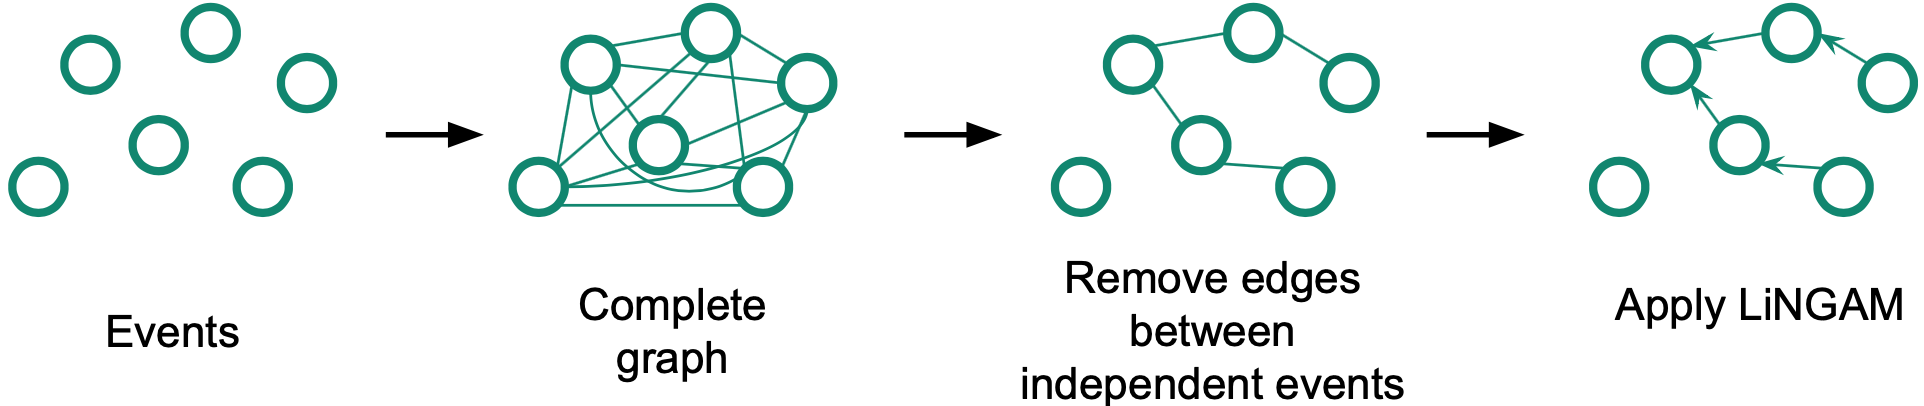
\includegraphics[width=\textwidth]{figures/fb_flow.png}
    \caption{The functional-based approach flow.}
\end{figure}
To apply this group of algorithms to our case, we first need to create the graph skeleton with a PC algorithm (see also Figure \hyperref[fig:fb-flow]{10}). Then, we estimate the orientation of edges based on the data asymmetry effect. Kobayashi et al. \cite{jarry2021quantitative} found that MixedLiNGAM discovers ten times more causal edges than the PC algorithm. 
\subsection{The Granger Causality}
\begin{figure}[ht]
\centering
    \label{fig:granger}
    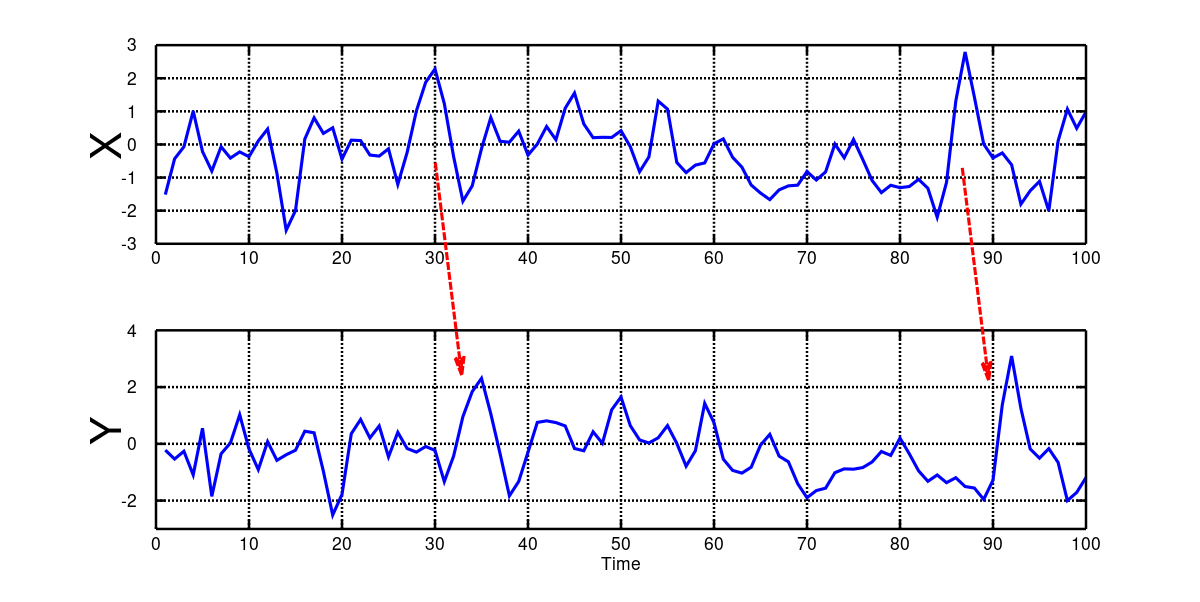
\includegraphics[width=\textwidth]{figures/granger.png}
    \caption{The time-series $X$ Granger-causes time-series $Y$.}
\end{figure}

The Granger causality test is a statistical hypothesis test for determining whether one time-series helps forecast another. Figure \hyperref[fig:fb-example]{11} is an example where the patterns in $X$ are approximately repeated in $Y$ after some time lag (two arrows). Thus, past values of $X$ can be used to predict future values of $Y$. Clive Granger defined the causality relationship based on two principles: the cause occurs before the effect, and the cause has unique information about the future values of its effect \cite{granger1980testing}.\newline

To test the Granger causality, we need to augment the autoregression model of one time-series $Y$ by including lagged values of another time-series $X$: 
\begin{equation}
y_{t}=c+\epsilon_{t}+\sum_{i=1}^{p} \alpha_{i} y_{t-i}+\sum_{i=1}^{p} \beta_{i} x_{t-i}
\end{equation}
So, we need to determine if any lags of $X$ are statistically significant in our model of $Y$. We can do this using a Wald test F-statistic for linear restrictions. The Wald test is based on the relatively simple premise that we wish to compare the performance of a restricted model for $Y$, which excludes $X$, against an unrestricted model for $Y$, which includes $X$. The null hypothesis that $X$ does not Granger-cause $Y$ is accepted if and only if no lagged values of $X$ are retained in the regression according to an F-statistic.\newline

However, Granger stressed that some studies using "Granger causality" testing in areas outside economics reached "ridiculous" conclusions. \textit{"Of course, many ridiculous papers appeared,"} he said in his Nobel lecture \cite{granger2004nobel}. Thus, the Granger causality is not the true causality. It provides no insight into the relationship between the variables and is helpful only in the forecasting case. Moreover, time is the key parameter in this approach. However, the timestamp of system logs or time-series is not always reliable for determining causal directions due to time synchronization errors between devices, jitter, and network failures \cite{kobayashi2017mining}. This kind of approach has other limitations. One is that the Granger causality only gives information about linear features. Besides this, one more is that the variables must be stationary. Finally, this approach depends on the observations we are dealing with \cite{seth2007granger}.
